% Oversells — o‘zbekcha darslik shabloni (XeLaTeX yoki LuaLaTeX bilan kompilyatsiya qiling).
% Default Oversells template: Uzbek Latin + Cyrillic textbook (compile with XeLaTeX or LuaLaTeX).
\documentclass[12pt,a4paper]{article}

% --- Sahifa va shriftlar / Page and fonts ---------------------------------
\usepackage[margin=2.5cm]{geometry}
\usepackage{fontspec}
% Noto Serif: Lotin va Kirill yozuvlarini (oʻ, gʻ, ʼ, ў, қ, ғ, ҳ) toʻliq qamraydi.
\setmainfont{Noto Serif}
\setsansfont{Noto Sans}
\setmonofont{DejaVu Sans Mono}

% --- Til / Language -------------------------------------------------------
% Asosiy til: oʻzbek (lotin); kirill matn uchun: \begin{otherlanguage}{uzbekcyr}.
% Main language: Uzbek (Latin); use the "uzbekcyr" language for Cyrillic text.
\usepackage{babel}
\babelprovide[import=uz-Latn, main]{uzbek}
\babelprovide[import=uz-Cyrl]{uzbekcyr}
% Oʻzbek tili uchun boʻgʻin koʻchirish qoidalari yoʻq — satrlarni moslashuvchan qilamiz.
% There are no Uzbek hyphenation patterns, so allow a bit more inter-word stretch.
\setlength{\emergencystretch}{3em}

% --- Matematika va grafika / Math and graphics ----------------------------
\usepackage{amsmath, amssymb, amsthm}
\usepackage{graphicx}
\usepackage{tikz}
\usetikzlibrary{babel}
\usepackage{pgfplots}
\pgfplotsset{compat=1.18}
\usepackage[hidelinks]{hyperref}

\newtheorem{teorema}{Teorema}
\newtheorem{misol}{Misol}
\theoremstyle{definition}
\newtheorem{tarif}{Taʼrif}

\title{Algebra va analiz asoslari}
\author{Muallif ismi}
\date{\today}

\begin{document}

\maketitle

% Kirish boʻlimi: alohida fayl sifatida \input orqali ulanadi.
\section{Kirish}

Ushbu hujjat \textbf{Oversells} platformasida yaratilgan namunaviy darslik
sahifasi. Oʻzbek lotin yozuvidagi maxsus harflar toʻgʻri koʻrinadi:
oʻquvchi, gʻalaba, maʼlumot, taʼlim, qoʻl, togʻ.

Matematik ifodalar uchun \texttt{amsmath}, chizmalar uchun \texttt{tikz}
va \texttt{pgfplots} paketlaridan foydalaniladi.


\section{Kvadrat tenglama}

\begin{tarif}
  $ax^2 + bx + c = 0$ \ ($a \neq 0$) koʻrinishidagi tenglama
  \emph{kvadrat tenglama} deb ataladi.
\end{tarif}

\begin{teorema}[Ildizlar formulasi]
  Agar $D = b^2 - 4ac \geq 0$ boʻlsa, tenglamaning ildizlari
  \begin{equation}\label{eq:ildiz}
    x_{1,2} = \frac{-b \pm \sqrt{D}}{2a}.
  \end{equation}
\end{teorema}

\begin{misol}
  $x^2 - 5x + 6 = 0$ tenglamani yeching. Bu yerda $D = 25 - 24 = 1$,
  demak \eqref{eq:ildiz} formulaga koʻra $x_1 = 2$, $x_2 = 3$.
\end{misol}

\section{Funksiya grafigi}

Quyida $y = x^2 - 5x + 6$ funksiyaning grafigi keltirilgan.

\begin{center}
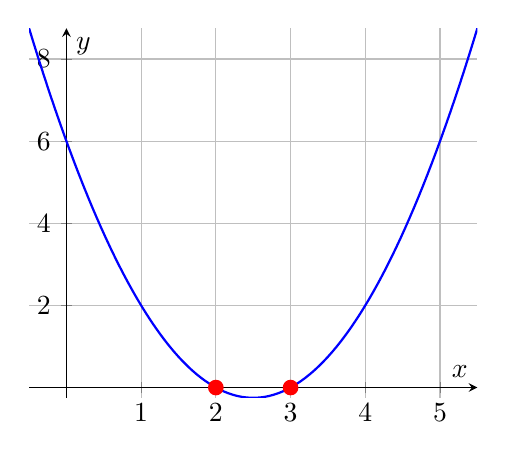
\begin{tikzpicture}
  \begin{axis}[
      axis lines = middle,
      xlabel = {$x$}, ylabel = {$y$},
      width = 0.6\textwidth,
      grid = both,
      samples = 100,
    ]
    \addplot[domain=-0.5:5.5, thick, blue] {x^2 - 5*x + 6};
    \node[circle, fill=red, inner sep=2pt] at (axis cs:2,0) {};
    \node[circle, fill=red, inner sep=2pt] at (axis cs:3,0) {};
  \end{axis}
\end{tikzpicture}
\end{center}

\section{Integral}

\[
  \int_0^1 x^2\,dx = \left.\frac{x^3}{3}\right|_0^1 = \frac{1}{3},
  \qquad
  \sum_{k=1}^{n} k = \frac{n(n+1)}{2}.
\]

\begin{otherlanguage}{uzbekcyr}
\section{Кирилл ёзувидаги бўлим}

Ўзбек тилидаги матн кирилл ёзувида ҳам тўғри кўринади: ўқувчи, ғалаба,
қалам, ҳисоб. Масалан, $a^2 + b^2 = c^2$ — Пифагор теоремаси.
\end{otherlanguage}

\end{document}
